\section{Établir un modèle de données}
    \subsection{Réalisation d'un échantillon des données}

La préparation des données du projet \COREL s'effectue en coopération avec le prestataire. En effet, la société Data Futures est le gestionnaire de la plateforme d'annotation dans laquelle les chercheurs saisissent les données manquantes pour le projet, notamment les dates de début de période d'application des lois et les liens d'association et/ou d'association dirigée entre les lois. Ces informations sont présentes dans les annotations mais ont besoin d'être explicitées afin de pouvoir être ajoutées dans l'encodage : il est nécessaire d'ajouter des dates de fin d'application des lois notamment. L'équipe du projet a donc fait appel au prestataire afin de générer automatiquement les dates de fin de validité des lois à partir des liens de généalogie. Lorsqu'une loi en remplace une autre, la date de promulgation de la nouvelle loi marque la fin de l'application de la précédente. La chaîne de traitement des données est donc la suivante : les chercheurs enrichissent les données des annotations et les corrigent ; le prestataire génère automatiquement les dates de fin de validité des lois pour obtenir des bornes chronologiques ; les données sont ajoutées à l'encodage \TEI. Lors du stage, la première étape de cette chaîne de traitement était en cours de réalisation. La deuxième étape, prévue dans le calendrier du projet, indique que le prestataire fournit les données via des fichiers \JSON au mois de septembre. 

Afin d'anticiper la dernière étape de préparation des données, un échantillon des données a été réalisé sur un extrait du \dc, chapitre 6, section 25, \lu 254 et \li 1. Cet échantillon permet d'encoder les données manquantes afin d'établir le modèle d'encodage qui sera utilisé pour ajouter les données \JSON en \TEI. Dans un premier temps, il a été nécessaire d'identifier tous les types de données à ajouter et de déterminer les éléments \TEI les plus pertinents pour encoder ces informations. Cette étape a été réalisée une fois les documents \XML transformés en \TEI. Pour mener à bien le projet, il est pertinent d'ajouter dans l'encodage : 
\begin{itemize}
    \item Les bornes chronologiques pour chaque \lu et \li.
    \item Le lien vers les numérisations des textes.
    %à vérifier : est-ce que j'ai parlé au début du fait qu'on veut inclure les numérisations dans le site web, dans un visualiseur 3IF ?? mais que les ressources ne sont pas accessibles en ligne et que on ne peut pas accéder aux manifestes ? (et que l'équipe du projet ne le souhaite pas ?????)
    \item Un identifiant unique pour chaque \lu et \li permettant d'identifier dans chaque texte les lois associées.
    \item Des commentaires supplémentaires (de nature différente des commentaires officiels).
    \item L'enrichissement des données sur les entités nommées.
\end{itemize}

Ces éléments ont été choisis conjointement avec les chercheurs afin d'obtenir en résultat une édition en ligne complète et exploitable pour les chercheurs. À partir de cette liste, un modèle d'encodage à suivre a pu être mis en place. 

\begin{minted}{xml}
    <div type="substatute" n="1" xml:id="DQLL_254_1" 
         notBefore="1833" notAfter="1870">
        <pb  
        facs="https://duli-cunyi.freizo.org/mirador/book.cgi?catno=28941&amp;
        canvas=https://iiif.duli-cunyi.freizo.org/image/28941/canvas/p5"/>
            <p>一、反逆案内律應問擬凌遲之犯,其子孫訊明,
            實係不知謀逆情事者,無論已未成丁,均解交内務府閹割,發往新疆等處,
            給官兵為奴。如年在十歲以下者,牢固監禁,俟年届十一歲時,再行解交内務府,
            照例辦理。内務府大臣遇有解到閹割人犯,即遴派司員認眞看驗,並出具無弊切結,
            送交刑部,再行覆驗。如有情弊,即行奏參,務須查驗明確,再交兵部,發往新疆,
            給官兵為奴。至其餘律應緣坐男犯,並非逆犯子孫,年在十六歲以上者,
            發往新疆等處,給官兵為奴。如年在十五歲以下者,牢固監禁,
            俟成丁時再行發遣。緣坐婦女,發各省駐防,給官員兵丁為奴。
            其知情不首干連人犯,仍依律擬流。</p>
            <note type='metadata'>Notes on the law</note>
    </div>
\end{minted}

\subsubsection{Liens vers les images}
Les liens vers les images peuvent être ajoutés via l'attribut \texttt{@facs} sur les balises \texttt{<pb/>} qui indiquent le début d'une nouvelle page. Ces balises ont été ajoutées aux sources numériques afin de faciliter la pagination de l'édition numérique et permettra d'afficher l'image en regard du texte. Le projet \COREL souhaite aboutir à une éditon simple qui propose le texte et l'image correspondante à la page près. Un facsimile interactif n'est pas envisagé, c'est pourquoi seul l'attribut \texttt{@facs} a été choisi pour intégrer les images à l'encodage. Cette solution a également été adoptée pour le projet \cordel : 
\begin{minted}{xml}
     <div>
        <pb n="1" source="Moreno_001_1.jpg" 
        facs="fedora_ug8110021/full/full/0/default.jpg"/>
\end{minted}

L'intégration des images pose toutefois un problème d'\textit{open access} qui n'a pas pu être résolu dans le cadre de mon stage. En effet, l'équipe du projet ne dispose pas des liens \IIIF des images, contrairement au projet \cordel. Une \URL \IIIF accepte plusieurs paramètres qui permettent d'afficher différentes zones de l'image à partir des pixels. Dans l'exemple du projet \cordel, l'image est affichée en entier grâce au paramètre \texttt{full}. \footnote{Ressource image issue de l'article \og C'est quoi le IIIF ? \fg de l'Université de Genève.} Les liens \IIIF des numérisations des codes légaux, de même que les liens des ressources images seules (indiquées dans les fichiers \JSON en tant qu'identifiant), ne sont pas disponibles sur le web. Le prestataire ne fournit que le lien permettant d'accéder à l'image via leur serveur. Cela pose un problème d'accessibilité, en cours de résolution par l'équipe du projet, afin que les numérisations soient librement accessibles sur le web et que les liens puissent être inclus dans l'édition numérique. Dans l'échantillon, il a été décidé d'inclure le lien présent dans les fichiers \JSON, bien qu'il ne soit pas accessible pour le moment. Une fois l'accès autorisé par le prestataire, utiliser les liens des fichiers \JSON permettra d'automatiser l'ajout des liens dans l'encodage via un script. Cette solution est la plus satisfaisante pour le projet, étant donné que la majorité des informations à ajouter doivent l'être depuis les fichiers \JSON. 

\begin{figure}
    \centering
    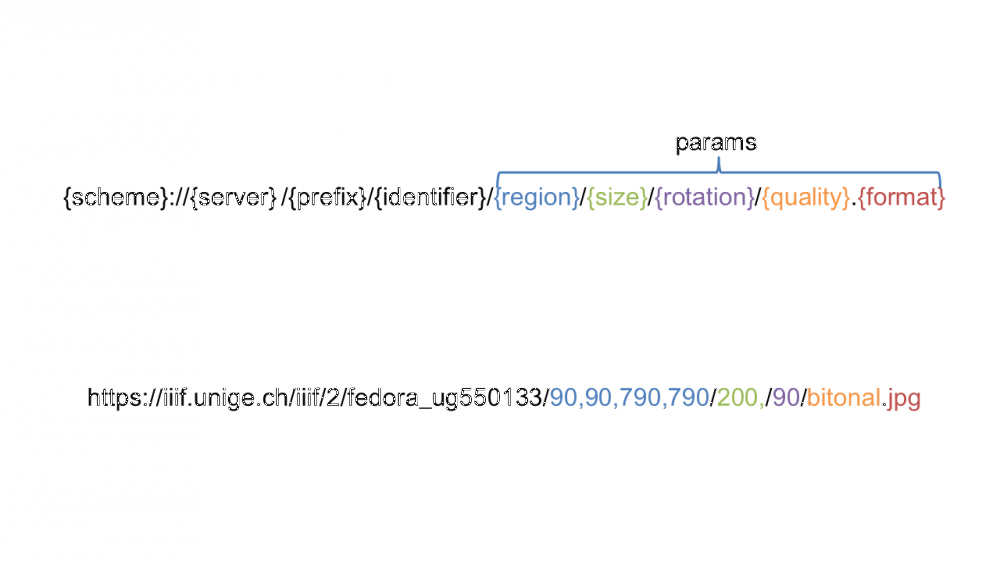
\includegraphics[width=\textwidth]{images/iiif.png}
    \caption{Schéma explicatif d'une \URL \IIIF}
\end{figure}

\subsubsection{Les bornes chronologiques et les identifiants \XML}
L'ajout des bornes chronologiques est également permis par des attributs \TEI. Sur chaque \lu et \li, contenues dans des éléments \texttt{<div>}, il est possible d'ajouter des attributs \texttt{@notBefore} et \texttt{@notAfter} afin d'ajouter les dates à l'encodage. Toutefois, cet ajout demande un élargissement des règles de la \TEI car ces attributs ne sont pas autorisés sur des éléments \texttt{<div>}. L'ajout de ces attributs est indispensable afin de reconstituer la législation pour une année donnée. Placer ces attributs sur les balises \texttt{<div>} est nécessaire afin de pouvoir afficher la loi contenue dans cette balise afin de créer le \cv, c'est pourquoi la modification de la \TEI a été choisie pour cet élément. En plus de ces bornes chronologiques, l'élément \texttt{<div>} contient l'attribut \texttt{@xml:id} qui permet d'attribuer à chaque loi un identifiant unique. Cela permet de faire le lien avec les fichiers \JSON et d'attribuer aux lois associées, c'est-à-dire les lois qui sont les mêmes d'un texte à un autre, le même identifiant. 

Les données à inclure dans les attributs font le lien entre le format \XML et le format \JSON. Toutefois, d'autres informations d'enrichissement des données doivent être ajoutées. 

\subsubsection{Les commentaires et les entités nommées}
Les commentaires et les entités nommées sont des informations additionnelles, qui ne sont pas présentes dans les annotations. En effet, les commentaires ont été océrisés mais n'ont pas été ajoutés dans l'encodage \XML du projet \LSC, ni dans les annotations. Quelques informations sur les entités nommées ont été ajoutées dans les annotations, toutefois elles restent partielles et n'ont pas été corrigées. 

Plusieurs types de commentaires existent dans les textes de lois chinois. Les commentaires officiels, rédigés en même temps que le texte de loi, sont déjà présents dans l'encodage dans des éléments \texttt{<note type='official'>}. Ils apparaissent dans les sources originales dans une police de caractère légèrement inférieure. Sur le site web \LSC, l'affichage met en valeur ces commentaires avec une couleur différente du reste du texte. D'autres commentaires, notamment d'auteurs ayant rédigés les compilations, seront ajoutés à l'édition en ligne. Elles sont représentées dans l'échantillon par des balises \texttt{<note>}, toutefois leur type n'a pas encore été défini. À des fins explicatives, un attribut \texttt{@type} a été ajoutés sur ces balises pour indiquer que chaque commentaire doit posséder cet attribut obligatoire, avec un type défini.

De plus, des commentaires qui ne sont pas présents dans l'\OCR peuvent également être ajoutés, afin de créer dans l'édition en ligne un mode \og métadonnées \fg qui permettrait d'afficher des informations supplémentaires sur les lois. Ces commentaires ont donc un attribut \texttt{@type='metadata'}. 

Par ailleurs, l'équipe du projet souhaite également enrichir les informations sur les entités nommées, afin d'envisager dans l'édition en ligne un mode \og entités nommées \fg pour les mettre en avant. Dans l'encodage \LSC, les entités nommées sont balisées par des éléments \texttt{<personname>} ou \texttt{<propername>}. Le projet \COREL souhaite encoder un peu plus précisément les noms de personnes en leur ajoutant notamment un nom de rôle : 

\begin{minted}{xml}
    <persName role="governor" ref="#覺羅伍拉納">
        <roleName>福建巡撫</roleName>
        <name>覺羅伍拉納</name>
    </persName>
\end{minted}
En effet, la plupart des personnes mentionnées sont des fonctionnaires et ont donc un rôle qui peut être mis en valeur dans l'encodage. Afin d'éviter les erreurs d'encodage et de garantir sa régularité, il est pertinent d'ajouter dans le \texttt{<teiHeader>} les informations relatives à ces entités nommées dans un élément \texttt{<listPerson>} : 

\begin{minted}{xml}
     <listPerson>
        <person xml:id="覺羅伍拉納">
            <persName role="governor" ref="#覺羅伍拉納">
                <roleName>福建巡撫</roleName>
                <name>覺羅伍拉納</name>
            </persName>
            <note>Biographical information</note>
        </person>
        <person xml:id="何東山">
            <persName role="party" ref="#何東山">
                     何東山
            </persName>
            <note>Biographical information</note>
        </person>
        <person xml:id="何適">
            <persName role="party" ref="#何適">
                     何適
            </persName>
            <note>Biographical information</note>
        </person>
    </listPerson>
\end{minted}
Lister les entités nommées dans le \texttt{<teiHeader>} permet de les identifier grâce à un attribut \textit{@xml:id} et donc d'afficher les informations relatives à chaque entité nommée si un mode \og entités nommées \fg est créé pour le site web. Le lien entre l'identifiant \XML et le nom de personne dans l'encodage s'effectue grâce à l'attribut \texttt{ref.} Le modèle d'encodage des entités nommées a pu être déterminé grâce à l'exemple du projet \disco de l'INRIA. En effet, leur projet accorde une place importante aux entités nommées puisqu'ils offrent une édition numérique de correspondances : 
\begin{minted}{xml}
     <listPerson>
        <person xml:id="p0001">
            <persName>d'Estournelles de Constant, Paul</persName>
            <persName>
                <roleName type="nobility">Baron</roleName>
                <forename>Paul</forename>
                <nameLink>d'</nameLink>
                <surname>Estournelles de Constant</surname>
            </persName>
            <persName>Paul Henri Balluet d'Estournelles de Constant</persName>
            <nationality>French</nationality>
            <birth>
                <date when-iso="1852-11-22"/>
                <placeName>La Flèche (Sarthe)</placeName>
            </birth>
            ...
        </person>
    </listPerson>
\end{minted}
L'édition en ligne de \disco offre un encodage exhaustif des entités nommées, dans un fichier d'index \TEI dédié à cet usage. Dans le cadre du projet \COREL, un fichier d'index n'est pas envisagé pour le moment étant donné que le corpus est constitué d'un nombre restreint de documents et que les entités nommées ne sont pas le centre du projet. Toutefois, la liste des entités nommées pourra être transposée dans un index si l'encodage s'enrichit et donne lieu à une liste et à des informations exhaustives. Pour ajouter des informations additionnelles pour chaque entité nommée, l'échantillon propose une balise \texttt{<note>} pour ajouter des informations biographiques, sans structure prédéfinie, qui pourront être affichées dans le mode \og entités nommées \fg. 

Pour le balisage des noms de lieux, une structure similaire a été mise en place dans l'échantillon. Une liste des lieux est présente dans le \texttt{<teiHeader>} : 
\begin{minted}{xml}
     <listPlace>
        <place xml:id="寧古塔">
            <placeName ref="#寧古塔">
                寧古塔
            </placeName>
            <note>Information about the place</note>
        </place>
    </listPlace>
\end{minted}
À l'instar des noms de personnes, le nom du lieu possède un identifiant unique qui permet de le lier au balisage présent au sein du texte et un élément \texttt{<note>} afin d'ajouter des informations supplémentaires sur le lieu. Les noms de lieux sont mentionnés dans les textes de loi en tant que lieu d'où provient l'origine de la loi ou bien en tant que lieu d'application. Selon le contexte, la balise \texttt{<placeName>} porte donc l'attribut \texttt{@type} avec pour valeur \texttt{'application'} ou \texttt{'origin'}. 

L'établissement d'un échantillon des données permet ainsi de fournir un modèle d'encodage à suivre pour la suite du projet et donne un aperçu de l'état final du jeu de données \TEI. L'exercice a pu mettre en valeur les difficultés qui peuvent être rencontrées lors de l'encodage, notamment l'accessibilité des ressources ou le besoin d'étendre la \TEI, et ainsi de les anticiper et de commencer à les résoudre en amont afin de pouvoir enrichir le jeu de données dès le mois de septembre. Toutefois, il est également pertinent d'étudier les limites de cet aperçu idéalisé des données.

\subsection{Limites de cet aperçu idéalisé des données}

§ Paragraphe 1

Idée :\\
Exemple :\\
Référence :\\
Transition :\\

§ Paragraphe 2

Idée :\\
Exemple :\\
Référence :\\
Transition :\\

§ Paragraphe 3

Idée :\\
Exemple :\\
Référence :\\
Transition :\\


 \section{Un schéma d’encodage}
    \subsection{La documentation de l’encodage}

§ Paragraphe 1

Idée :\\
Exemple :\\
Référence :\\
Transition :\\

§ Paragraphe 2

Idée :\\
Exemple :\\
Référence :\\
Transition :\\

§ Paragraphe 3

Idée :\\
Exemple :\\
Référence :\\
Transition :\\

\subsection{Le schéma de validation}

§ Paragraphe 1

Idée :\\
Exemple :\\
Référence :\\
Transition :\\

§ Paragraphe 2

Idée :\\
Exemple :\\
Référence :\\
Transition :\\

§ Paragraphe 3

Idée :\\
Exemple :\\
Référence :\\
Transition :\\

